\documentclass{article}


\usepackage{PRIMEarxiv}

\usepackage[utf8]{inputenc} % allow utf-8 input
\usepackage[T1]{fontenc}    % use 8-bit T1 fonts
\usepackage{hyperref}       % hyperlinks
\usepackage{url}            % simple URL typesetting
\usepackage{booktabs}       % professional-quality tables
\usepackage{amsfonts}       % blackboard math symbols
\usepackage{nicefrac}       % compact symbols for 1/2, etc.
\usepackage{microtype}      % microtypography
\usepackage{lipsum}
\usepackage{fancyhdr}       % header
\usepackage{graphicx}       % graphics
\graphicspath{{media/}}     % organize your images and other figures under media/ folder

%Header
\pagestyle{fancy}
\thispagestyle{empty}
\rhead{ \textit{ }} 

% Update your Headers here
\fancyhead[LO]{Running Title for Header}
% \fancyhead[RE]{Firstauthor and Secondauthor} % Firstauthor et al. if more than 2 - must use \documentclass[twoside]{article}



  
%% Title
\title{Title Placeholder: The Physics \& Biology of Emergent Structures
%%%% Cite as
%%%% Update your official citation here when published 
\thanks{\textit{\underline{Citation}}: 
\textbf{Authors. Title. Pages.... DOI:000000/11111.}} 
}

% \author{
%   Author1, Author2 \\
%   Affiliation \\
%   Univ \\
%   City\\
%   \texttt{\{Author1, Author2\}email@email} \\
%   %% examples of more authors
%    \And
%   Author3 \\
%   Affiliation \\
%   Univ \\
%   City\\
%   \texttt{email@email} \\
%   %% \AND
%   %% Coauthor \\
%   %% Affiliation \\
%   %% Address \\
%   %% \texttt{email} \\
%   %% \And
%   %% Coauthor \\
%   %% Affiliation \\
%   %% Address \\
%   %% \texttt{email} \\
%   %% \And
%   %% Coauthor \\
%   %% Affiliation \\
%   %% Address \\
%   %% \texttt{email} \\
% }


\begin{document}
\maketitle


\begin{abstract}

\end{abstract}


% keywords can be removed
\keywords{Artificial life \and Representation learning \and Emergence \and Simulations}


\section{Introduction}

In science, a wide variety of problems require running simulations for obtaining the final results. 
For example, in physics, the \textit{no fast-forwarding theorem} states that a quantum system can't be simulated faster than its evolution according to time. 
However, if we only care about some macroscopic final properties, can we fast-forward or even skip simulation to abstract the spacetime to distill the macroscopic rules? 
Then, if we have the macroscopic rules, can we in turn use them to predict the microscopic rules? 
As an analogy, in our real world, physics could seen as the microscopic rules that govern the behavior of particles, while biology could be seen as the macroscopic rules that operate at the level of organisms. 
The question becomes: can we learn biology from physics, and vice versa? 
% This is similar to humans' System 1 thinking — e.g., when we drive cars, we humans don't run step-by-step simulations in our brains before we make decisions on next moves, 
% but rather, we run high-level simulations in the abstraction level, which allows us to predict from step $t$ to $t+\Delta t$, where $\Delta t$ might be large. Such macroscopic simulations correspond to "intuitive" physics, 
% which is imprecise but retains key information we want — this is in contrast to "real" physics that we employ in e.g. physical experiments.

This motivates the hypothesis that a good abstraction correlates with the capability to predicting macroscopic properties ahead of time. 
Specifically, a good abstraction might enable such capability, and/or predicting macroscopic properties ahead of time gives rise to a good abstraction. 
Once we have a good abstraction, that might encode enough information for us to learn the microscopic rules as well.

As a testbed, we picked an artificial life (ALife) substrate, Game of Life. The problem is: Can AI models trained on Game of Life's physics rules (step-by-step simulation) learn its biology (the emergent structures), and vice versa? 
Game of Life rules are easy to learn as they just involve convolution, but to predict the emergent structures is a much harder task, as the system is very chaotic and a tiny difference in initial state can result in very different states in several steps. 
% We show that models asked to predict more steps ahead contain better, i.e., more linearly separable, representation spaces.


\section{Related Work}

\subsection{Emergence}
Emergence refers to phenomena where some properties arise from a complex system that are not present when only looking at the individual components. There are many subfields of emergence, of which two ideas are highly relevant to our work.
\paragraph{Causal Emergence} The idea of causal emergence \cite{hoel_causal_2025} claims that macroscopic dynamics have more causal power than microscopic. 
For example, neurons in a human brain (microscopic) give rise to the emergent structure of the overall brain (macroscopic), 
and in turn, the brain can cause neurons to activate. 
In other words, the macroscopic structure that arises from emergence can in turn have more causal power on the microscopic structure. 
This might give us reason to believe that if we have macroscopic rules, we can predict the corresponding microscopic rules.
\paragraph{Computation \& Emergence} Crutchfield \cite{crutchfield_calculi_1994} claims that when emergence happens, the minimal program required to desctibe the system will both become shorter and switch to a new computational model. 
Take the emergent behavior of an ant colony as an example. The behavior of an individual ant is just random walk which can be described with a finite-state machine, and the program would be very long if we want to track each ant's state. 
If we instead consider the ant colony as a whole, ants prefer to follow stronger pheromone trails, and such behavior can be described with a pushdown automaton that would be much shorter, as it just needs to encode the pheromone map. 
Some work from causal emergence claims that when causal workings are maximized, time reversal symmetry, or reversibility, is maximized, which might be linked to the idea that the system can then be described with a shorter program.

\subsection{Hypernetworks}


\section{Methodology}

\subsection{Distill Game of Life ``Biology'' Rules}
Game of Life (GoL) has clear deterministic rules, and in particular, Conway's GoL is Turing-complete. 
Predicting the immediate next state ($t \rightarrow t+1$) is an easy task, but predicting multiple steps ahead ($t \rightarrow t+\Delta t$, where $\Delta t>1$) is a much harder task. 
Thus, we expect that a model has to make more mistakes and compress information more efficiently as $\Delta t$ increases. To test on a variety of simulations not limited to Conway's GoL, we also used other GoL rules found by the ASAL framework by \cite{kumar_automating_2024}.
\paragraph{Model}
We train ConvNet that maps from GoL state $t$ to state $t+\Delta t$ in one forward pass. Specifically, the ConvNet takes a 2D GoL grid as input, encodes it, and uses a $1 \times 1$ convolution to put it into a $D$-dimensional feature map. 
It adds a learned embedding for $\Delta t$, the number of timesteps skipped ahead, to each spatial location. Then, it applies a series of residual blocks. Finally, a $1 \times 1$ convolution projects back to the output channels.
\paragraph{Representation Space Evaluation}
To measure whether the ConvNet's representations capture the emergent structures in GoL, we use a linear probe from the representations of input GoL frame to CLIP vector encoding the frame. 
CLIP encoding could be seen as the average of lots of humans' representations, given its training data, so quantifying how well the representations linearly map to CLIP vectors is more objective than evaluation metrics such as how well the representations encode the number of gliders.

\subsection{Predict ``Biology'' from ``Physics''}

\subsection{Predict ``Physics'' from ``Biology''}


\section{Results}

\subsection{Distill Game of Life ``Biology'' Rules}
Preliminary results show that models asked to skip more timesteps ahead (higher $\Delta t$) have better representations of input states (states $t$), which is reflected as linear probe having higher $R^{2}$ to CLIP vector (as shown in the middle panel of Figure ~\ref{fig:7291_result}). 
The representations of target states (states $t+\Delta t$) don't necessarily improve as $\Delta t$ increases (as shown in the right panel of Figure ~\ref{fig:7291_result}). But when compared against the baseline of linear probing a random-weights model, the representations of target states do surpass the baseline's as dt increases.

\begin{figure}[h]
  \centering
  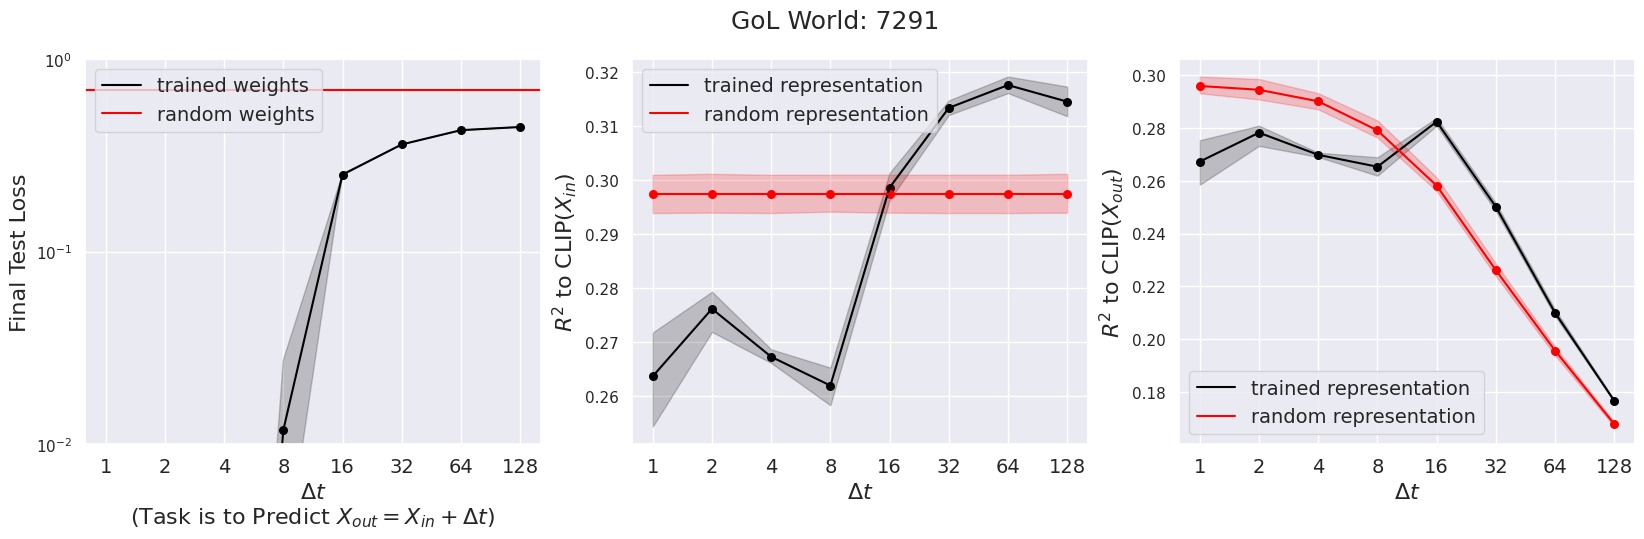
\includegraphics[width=\linewidth]{figures/7291_result.png}
  \caption{Results on Game of Life 7291. Left: ConvNet training result. Middle: Linear probe result for input state. Right: Linear probe result for target state.}
  \label{fig:7291_result}
\end{figure}

To analyze the quality of representations, we also visualize models' predictions. For example, Figure ~\ref{fig:7291_vis} below shows $\Delta t$ = 16 model's performance on GoL 7291. 
When comparing the model's prediction in the third row to the ground-truth target states in the second row, we can see that the model is learning to capture abstract patterns more confidently, without caring too much about predicting each cell precisely in the more chaotic regions.
As an analogy, the model captures the "organisms" in GoL, without caring too much about what molecules or atoms are present. This is exactly what we hope to see from a model that learns to capture the "emergent structures" of GoL.

\begin{figure}[h]
  \centering
  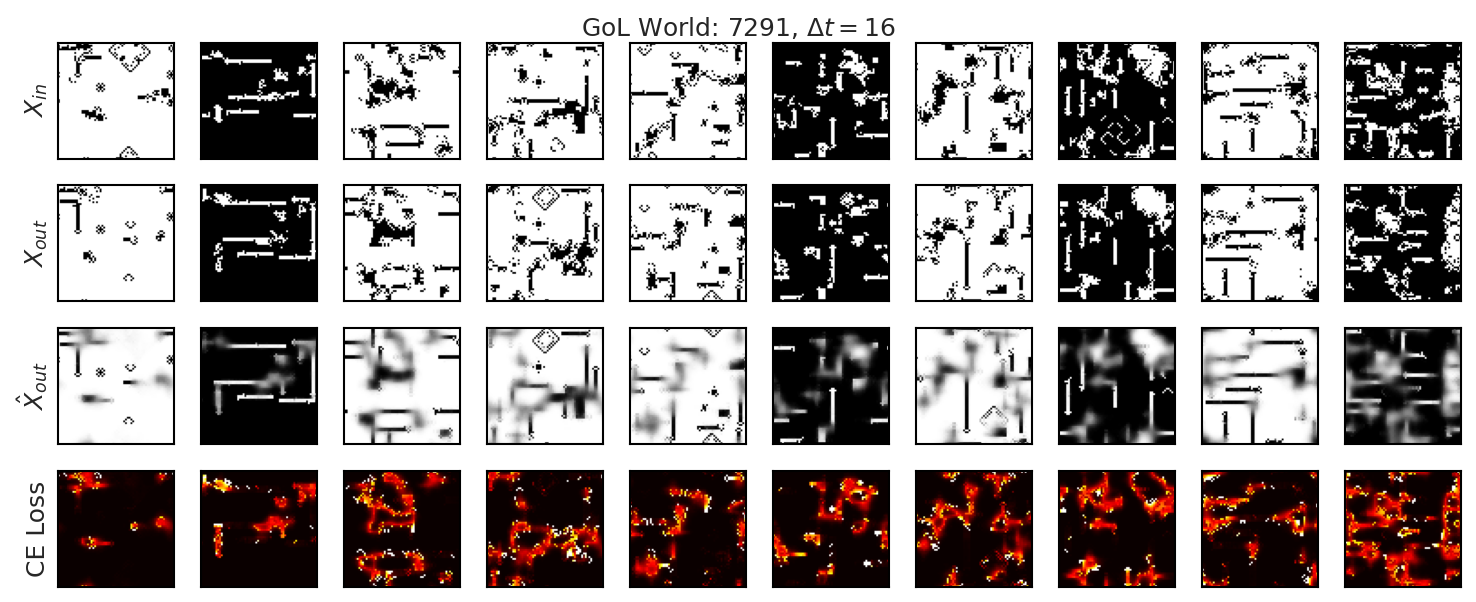
\includegraphics[width=\linewidth]{figures/7291_vis.png}
  \caption{Model performance on Game of Life 7291, with $\Delta t$ = 16. First row: Input state. Second row: Ground-truth target state. Third row: Model prediction of target state. Fourth row: Cross-entropy loss.}
  \label{fig:7291_vis}
\end{figure}

\subsection{Predict ``Biology'' from ``Physics''}

\subsection{Predict ``Physics'' from ``Biology''}


\section{Discussion}




%Bibliography
\bibliographystyle{unsrt}  
\bibliography{references}  


\end{document}
